\section{Zajęcia dydaktyczne --- sprawozdanie}
\subsection{Wprowadzenie}

Jak wspomniano wcześniej, zakres pracy inżynierskiej obejmuje przeprowadzenie zajęć laboratoryjnych opisanych w sekcji \ref{zajecia-dydaktyczne}.
Pierwsze zajęcia miały charakter testowy --- poza dydaktyką chciano: wychwycić potencjalne błędy w opracowanym symulatorze; sprawdzić czy studenci
potrafią zrealizować zadania laboratoryjne po przeczytaniu instrukcji; przygotować dyplomantów na problemy, które mogą pojawić się podczas prowadzenia
zajęć (awaria sprzętu, niekompatybilność oprogramowania na różnych systemach operacyjnych, niemożność zainstalowania oprogramowania ze względu na brakujące
biblioteki lub wersje bibiotek na komputerach). Problemy, które pojawiły się w trakcie pierwszych zajęć, zostały zaadresowane przez autorów, ażeby
ostateczna wersja była możliwie najlepsza.

\subsection{Przebieg zajęć}

Laboratoria odbyły się na wydziale ETI Politechniki Gdańskiej. Na początku zrealizowano wprowadzenie teoretyczne do omawianych zagadnień w postaci godzinnego
wykładu, który został przeprowadzony przez dyplomantów dla grupy studentów, pod okiem promotora.

Następnie podzielono studentów na dwie grupy: pierwsza odbyła zajęcia tego samego dnia, druga --- tydzień później.
Zajęcia rozpoczęto od wejściówki, a następnie zrealizowano zadania opracowane w ramach pracy.

W trakcie zajęć studenci wykonywali zadania samodzielnie, konsultując się przy tym między sobą. Autorzy niniejszej pracy
byli do ich dyspozycji, po to aby rozwiać wszelkie nieścisłości, nakierować studentów na właściwe rozwiązanie i tym podobne.

Uczestnicy zajęć mieli okazję zaznajomić się z zagadnieniami, które występują w warstwie fizycznej Ethernet, natomiast
opracowany symulator pomógł w wizualizacji tychże rozwiązań --- porównanie zachowania sygnału w przypadku różnych metod modulacji oraz
sprawdzenie działania i właściwości kodera Reeda-Solomona.


\begin{figure}[ht]
    \centering
    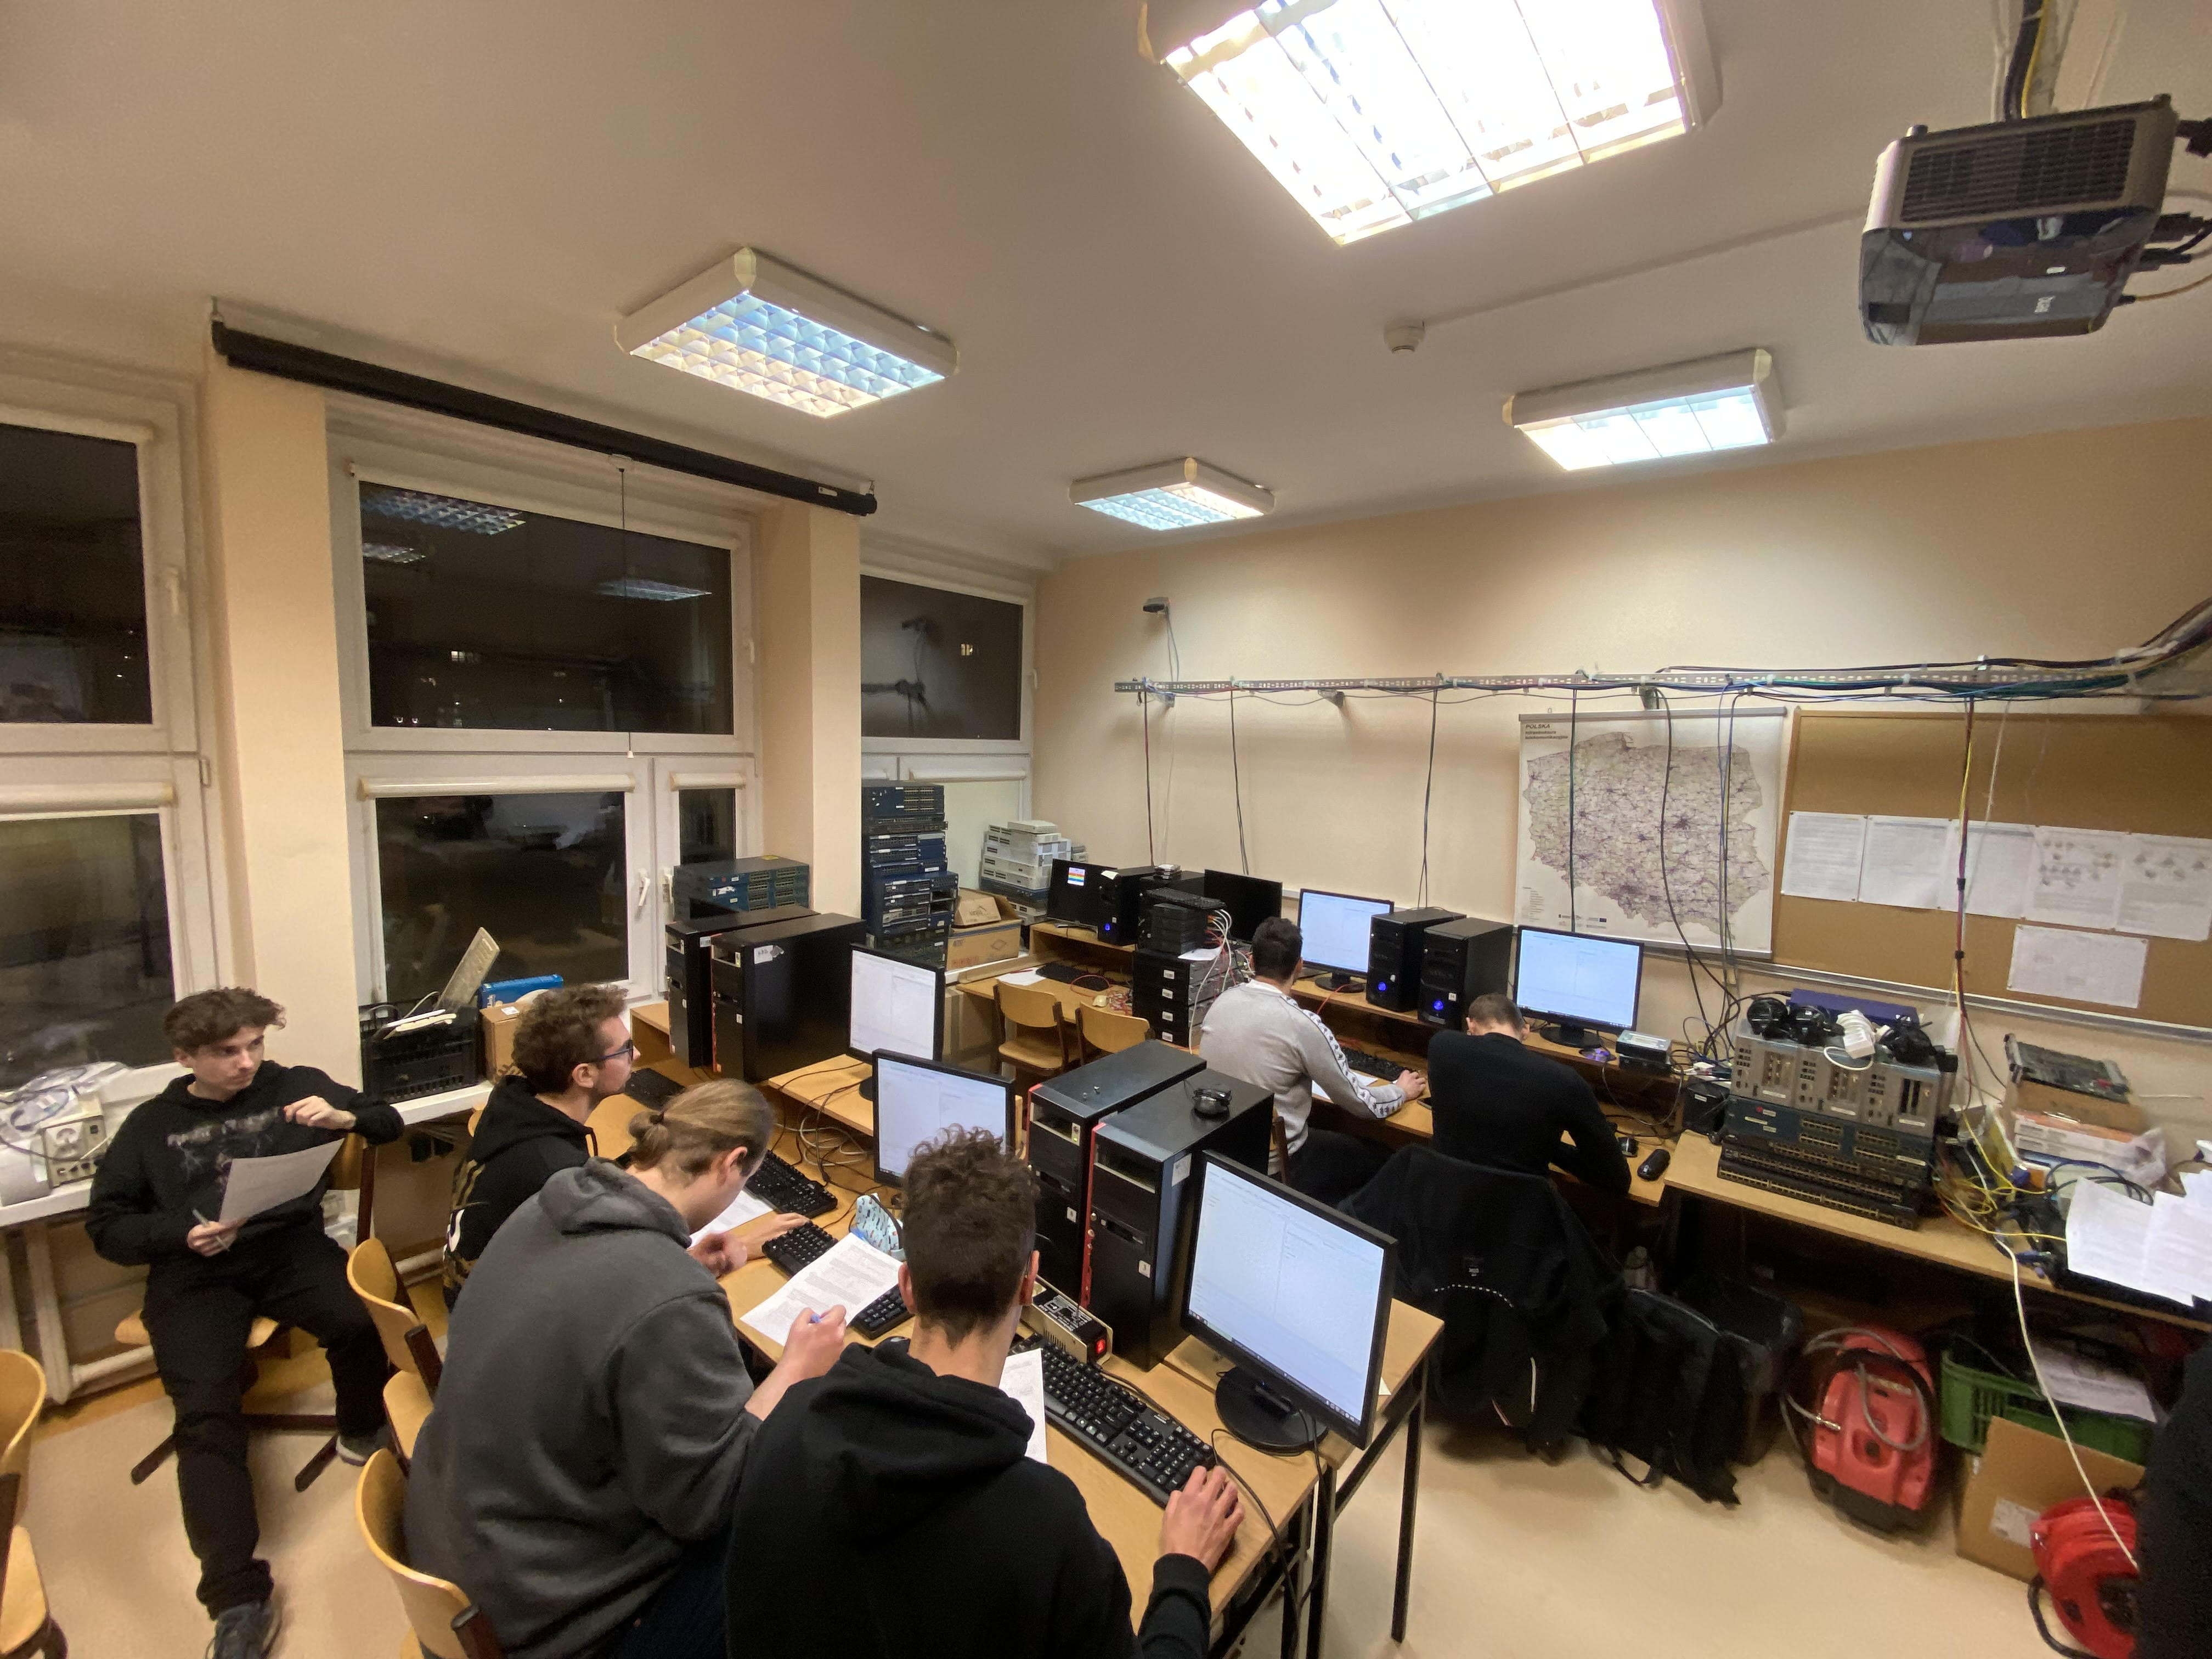
\includegraphics[width=\textwidth]{zajecia_lab.jpg}
    \caption{Zajęcia laboratoryjne}
    \label{fig:zajecia_lab_zdjecie}
\end{figure}
